\documentclass[a4paper]{article}
\usepackage{graphicx}
\usepackage{wrapfig}
\usepackage{caption}
\usepackage{subcaption}


\title{Selection Sort}
\author{Yarne Ramakers}
\date{\today}

\begin{document}

%\maketitle - had to comment as it took up too much space
\begin{center}
  Selection Sort \\
  Yarne Ramakers \\
  \today \\
\end{center}

\section{Introductie}
% Introduction to selection sort and its importance.

Selection sort is een simpel sorteeralgoritme dat een lijst sorteert door herhaaldelijk de kleinste (of grootste, afhankelijk van de sorteervolgorde) element uit de rest van de lijst te selecteren en dit vooraan te plaatsen.

\section{Bevindingen}
% Discuss the results of the experiments.
Mijn experimentele bevinding vertonen sterke overeenkomsten met het theoretische model van selection sort.
In de grafiek \ref{fig:selection-avg} toont de rode lijn de theoretische complexiteit van selection sort,
\begin{wrapfigure}{r}{0.5\textwidth}
  \begin{center}
    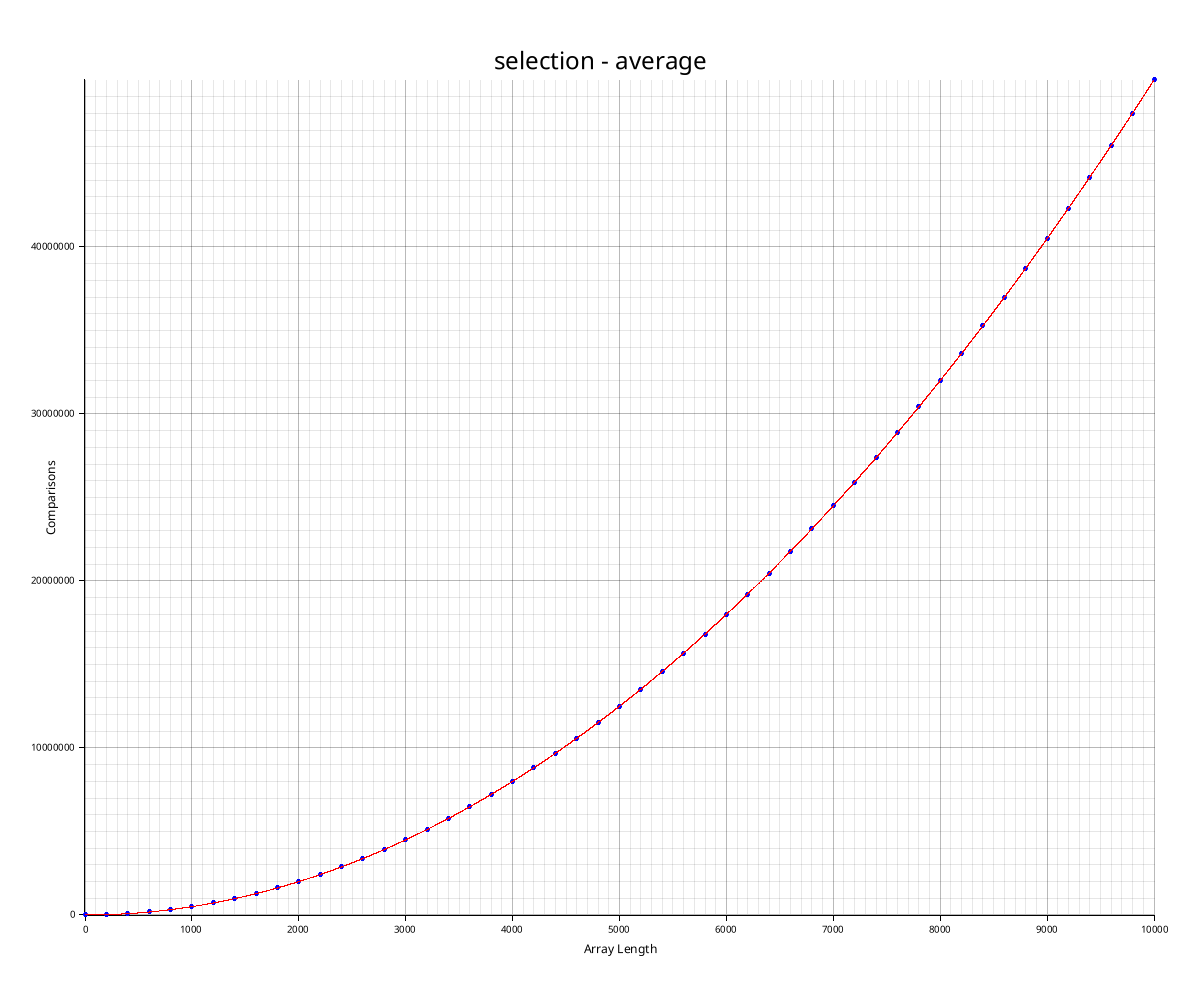
\includegraphics[width=0.48\textwidth]{../plots/selection-average.png}
    \caption{Average case}
    \label{fig:selection-avg}
  \end{center}
\end{wrapfigure}
namelijk $\sim \frac{1}{2} n^2$. 
En de blauwe punten tonen de gemeten vergelijkingen voor verschillende $n$. 
Deze $n$ is gekozen tussen 0 en 10 000 met een stapgrootte van 200.

\par

Voor lijsten met een kleinere $n$ is de gemeten complexiteit iets hoger dan de theoretische complexiteit.
Dit komt door de overhead van het meten van de complexiteit. Bij kleinere lijsten zullen de kleinere orde termen een grotere invloed hebben op de gemeten complexiteit.
Bij grotere $n$ is de gemeten complexiteit bijna gelijk aan de theoretische complexiteit.

\par

We maken hier geen onderscheid tussen een slechtse, gemiddelde of beste geval, omdat selection sort altijd $\sim \frac{1}{2} n^2$ vergelijkingen maakt.
Dit is ook te zien in de grafieken \ref{fig:selection-best} en \ref{fig:selection-worst} die respectievelijk de gemeten best en worst cases voorstellen.


\begin{figure}[h]
  \begin{subfigure}[b]{0.4\textwidth}
    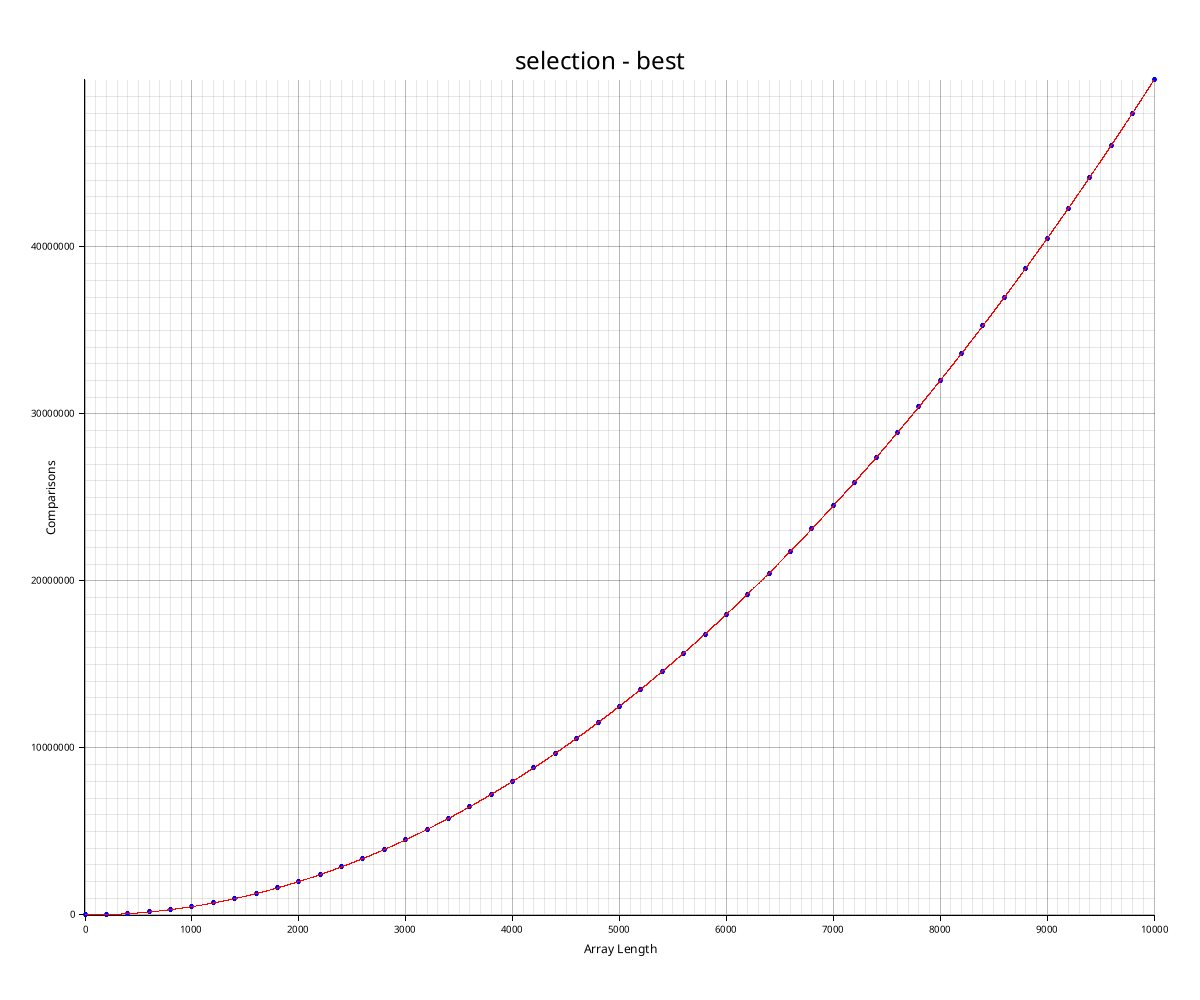
\includegraphics[width=\textwidth]{../plots/selection-best.png}
    \caption{Best case}
    \label{fig:selection-best}
  \end{subfigure}
  \begin{subfigure}[b]{0.4\textwidth}
    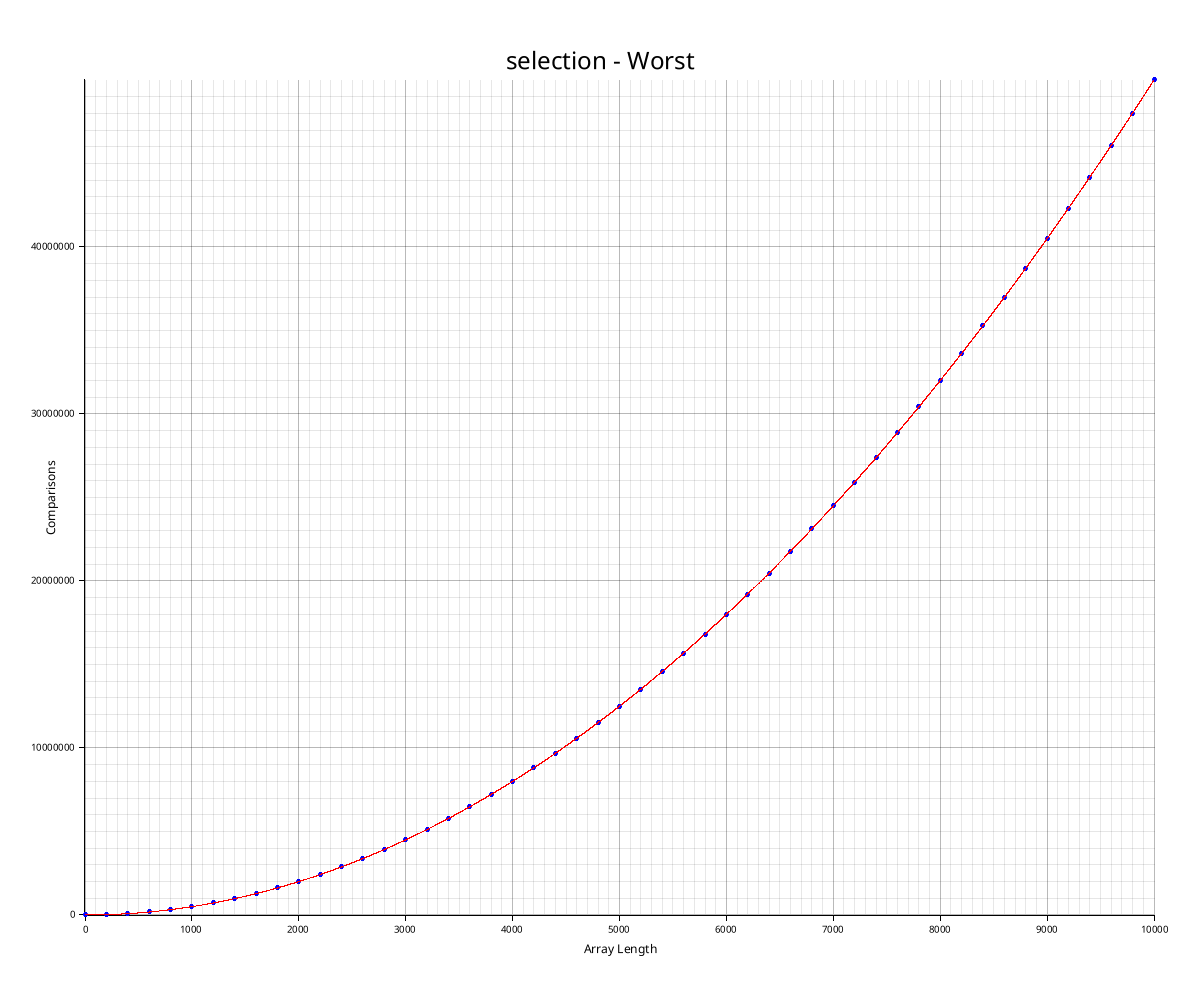
\includegraphics[width=\textwidth]{../plots/selection-worst.png}
    \caption{Worst case}
    \label{fig:selection-worst}
  \end{subfigure}
\end{figure}

\end{document}